\begin{frame}{Explications sur la sous-estimation}
  \begin{block}{Phénomènes non comptabilisés}
    \begin{itemize}
      \item Établissement du routage
      \item Acquittements (petit et non répétés)
      \item Pertes de paquets
    \end{itemize}
  \end{block}
  \begin{block}{Biais de mesure}
    \begin{itemize}
      \item Bootstrap du réseau non négligeable
    \end{itemize}
  \end{block}
\end{frame}

\begin{frame}{ContikiMAC timing}
  \begin{figure}
    \centering
    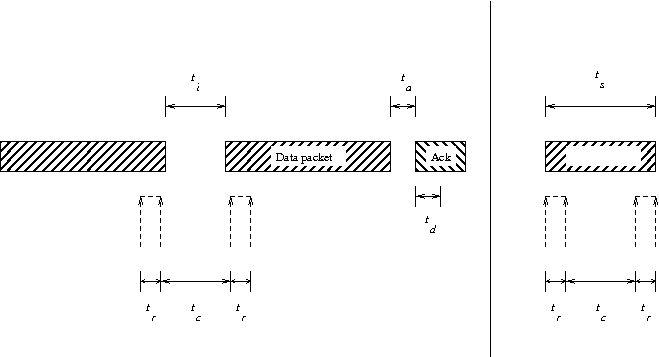
\includegraphics[width=\textwidth]{figures/contikimac_timing.png}
  \end{figure}
\end{frame}

\begin{frame}{Chaîne: Packet delivery ratio}
  \begin{figure}
    \centering
    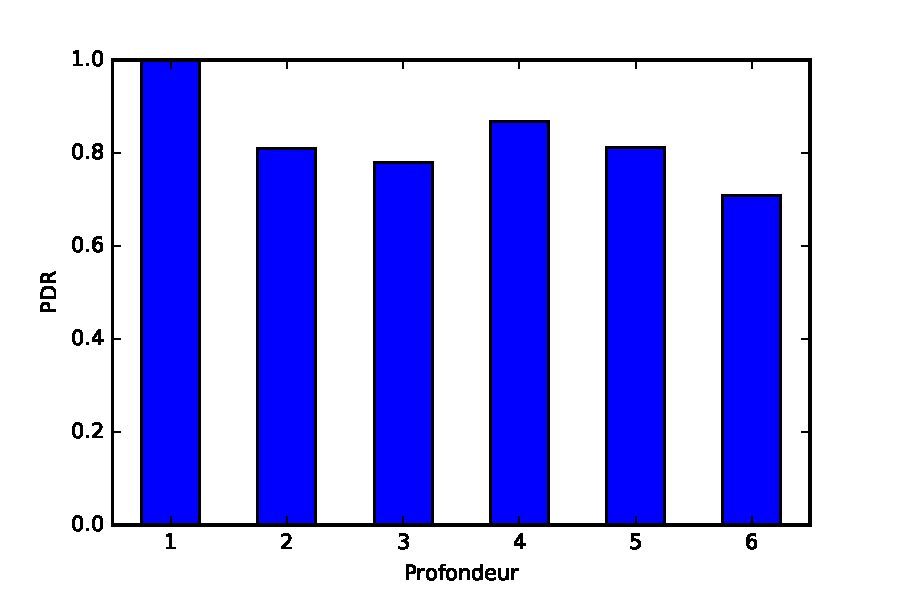
\includegraphics[width=\textwidth]{figures/new_pdr.pdf}
  \end{figure}
\end{frame}

\begin{frame}{$\delta(t)$ - Estimation ``étoilée'' - 1}
  \begin{figure}
    \centering  
    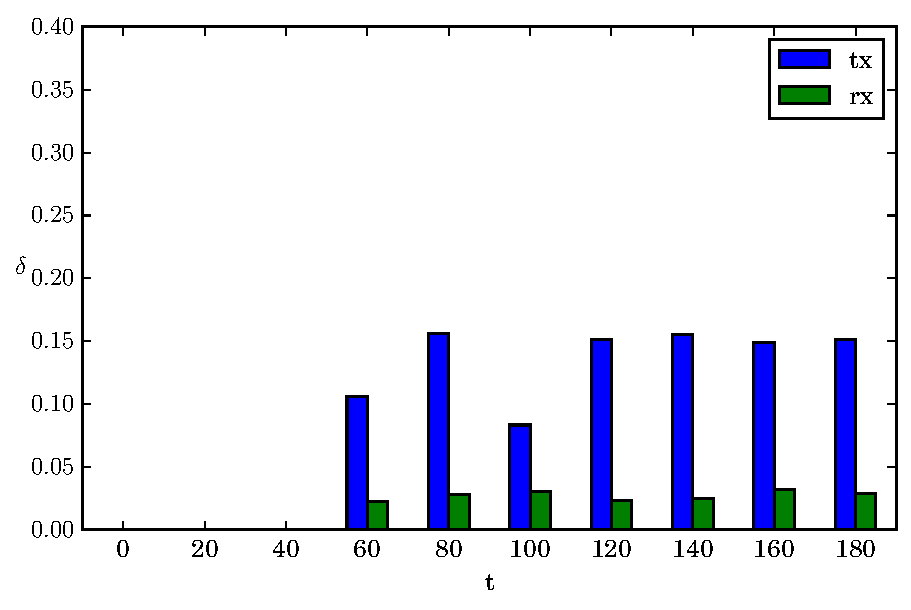
\includegraphics[width=\textwidth]{figures/evolution_noinfo_1.pdf}
  \end{figure}
\end{frame}

\begin{frame}{$\delta(t)$ - Estimation ``étoilée'' - 2}
  \begin{figure}
    \centering  
    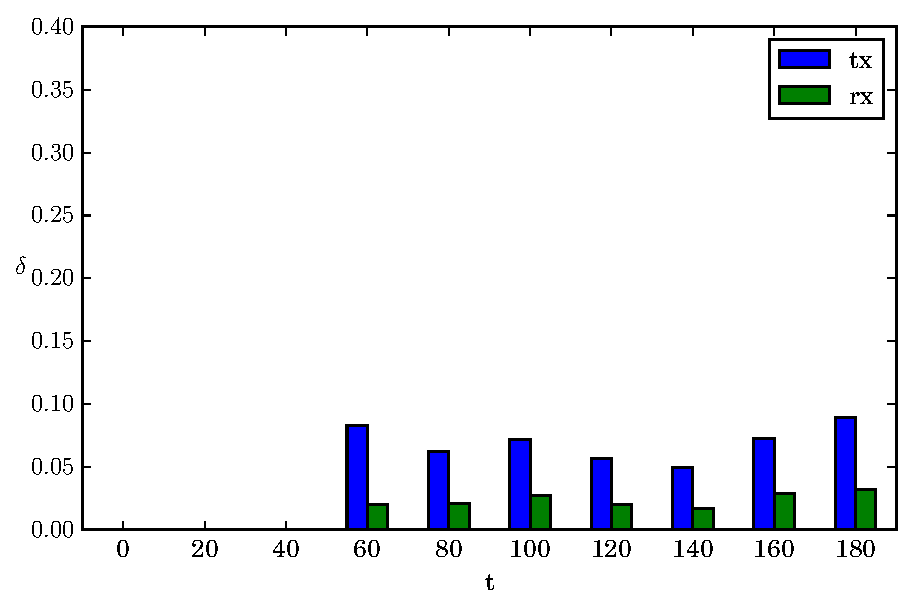
\includegraphics[width=\textwidth]{figures/evolution_noinfo_2.pdf}
  \end{figure}
\end{frame}

\begin{frame}{$\delta(t)$ - Estimation ``étoilée'' - 3}
  \begin{figure}
    \centering  
    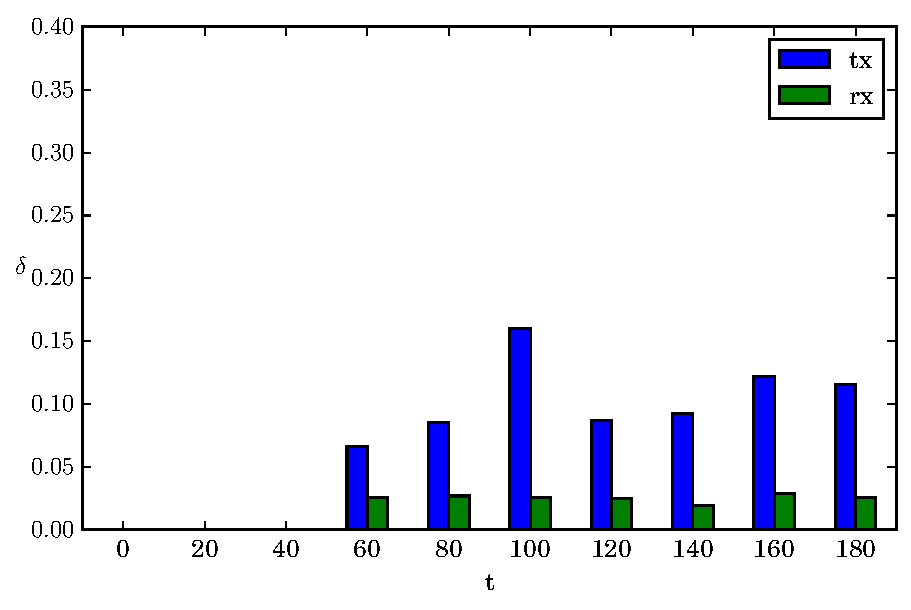
\includegraphics[width=\textwidth]{figures/evolution_noinfo_3.pdf}
  \end{figure}
\end{frame}

\begin{frame}{$\delta(t)$ - Estimation ``étoilée'' - 4}
  \begin{figure}
    \centering  
    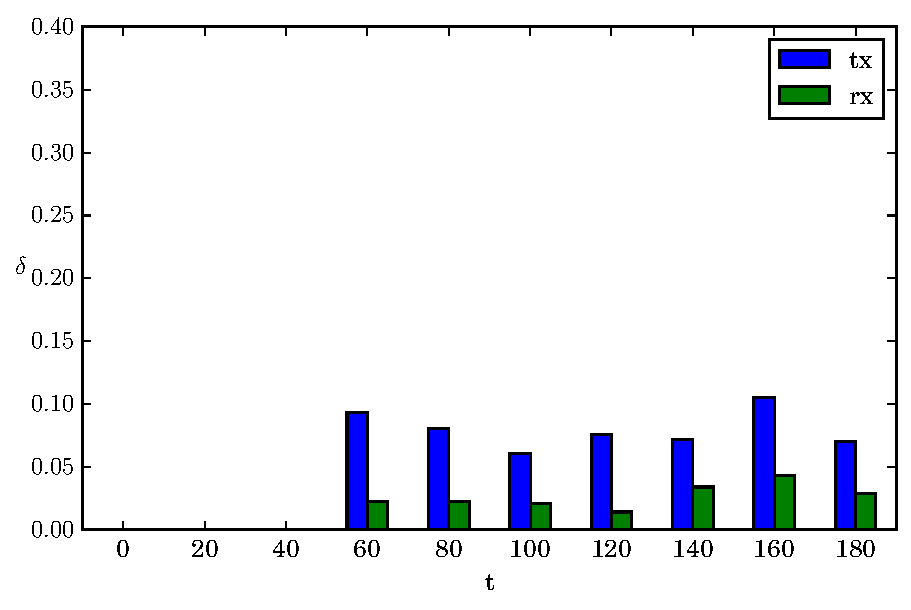
\includegraphics[width=\textwidth]{figures/evolution_noinfo_4.pdf}
  \end{figure}
\end{frame}

\begin{frame}{$\delta(t)$ - Estimation ``étoilée'' - 5}
  \begin{figure}
    \centering  
    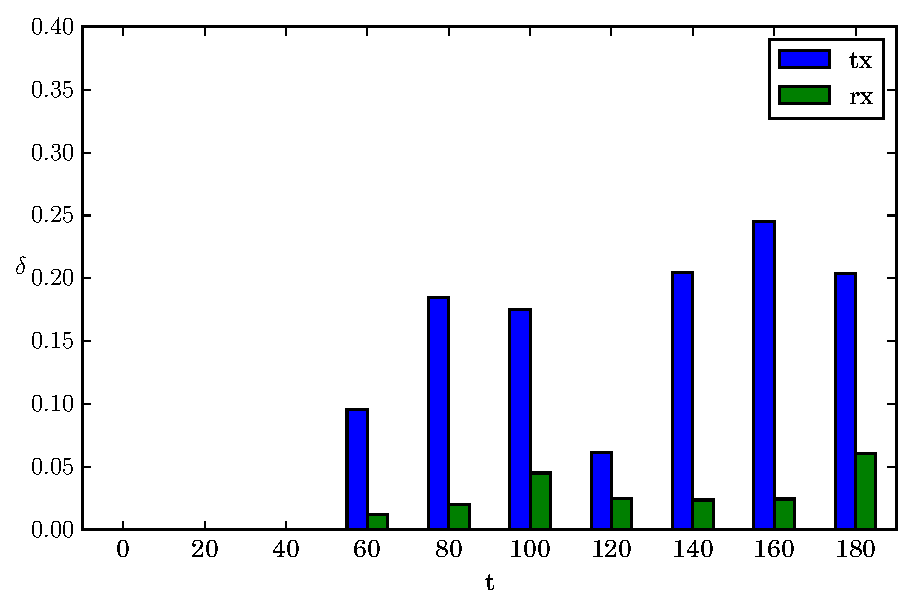
\includegraphics[width=\textwidth]{figures/evolution_noinfo_5.pdf}
  \end{figure}
\end{frame}

\begin{frame}{$\delta(t)$ - Estimation ``étoilée'' - 6}
  \begin{figure}
    \centering  
    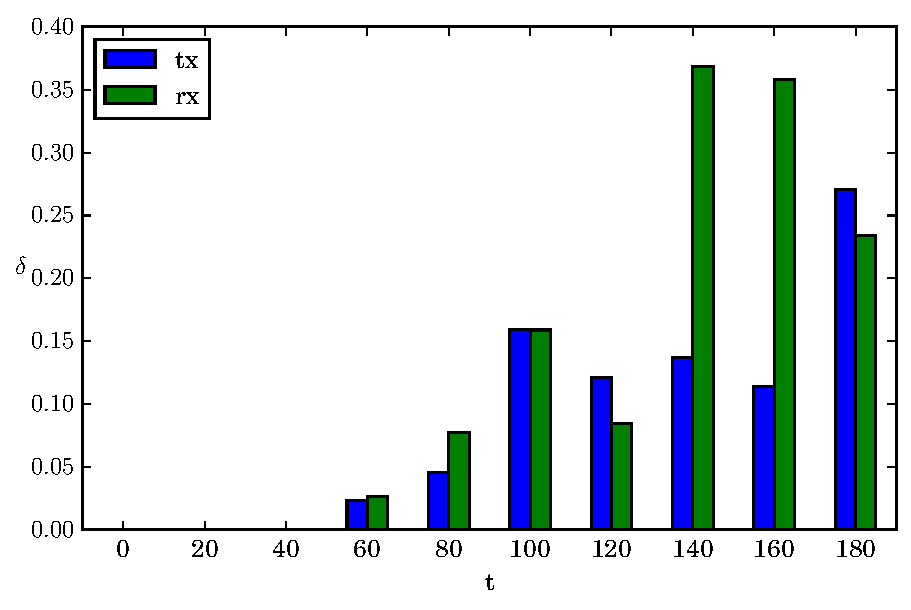
\includegraphics[width=\textwidth]{figures/evolution_noinfo_6.pdf}
  \end{figure}
\end{frame}

%%%%%%%%%%%%%%%%%%%%%%%%%%%%%%%%%%%%%%%%%%%%%%%%

\begin{frame}{$\delta(t)$ - Estimation ``maillée'' - 1}
  \begin{figure}
    \centering  
    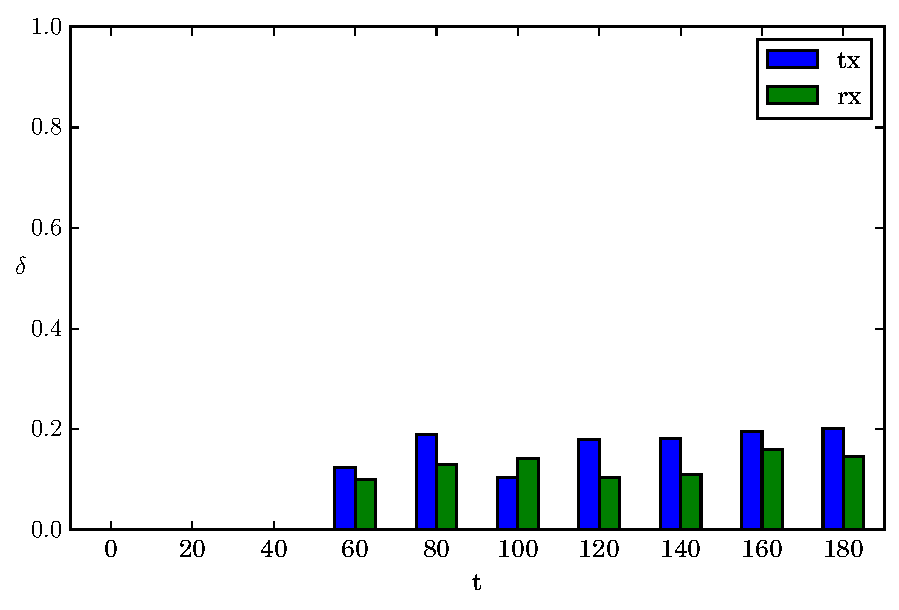
\includegraphics[width=\textwidth]{figures/evolution_route_1.pdf}
  \end{figure}
\end{frame}

\begin{frame}{$\delta(t)$ - Estimation ``maillée'' - 2}
  \begin{figure}
    \centering  
    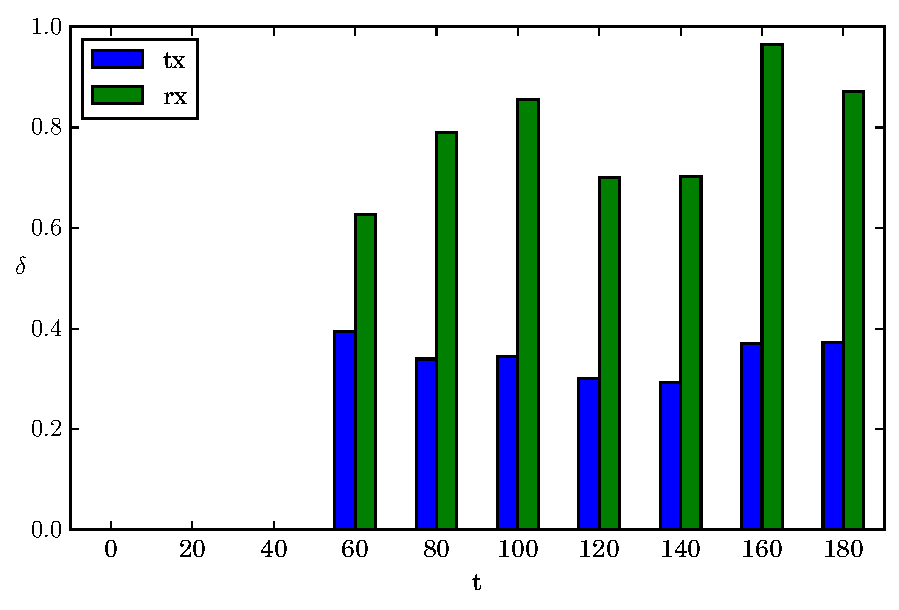
\includegraphics[width=\textwidth]{figures/evolution_route_2.pdf}
  \end{figure}
\end{frame}

\begin{frame}{$\delta(t)$ - Estimation ``maillée'' - 3}
  \begin{figure}
    \centering  
    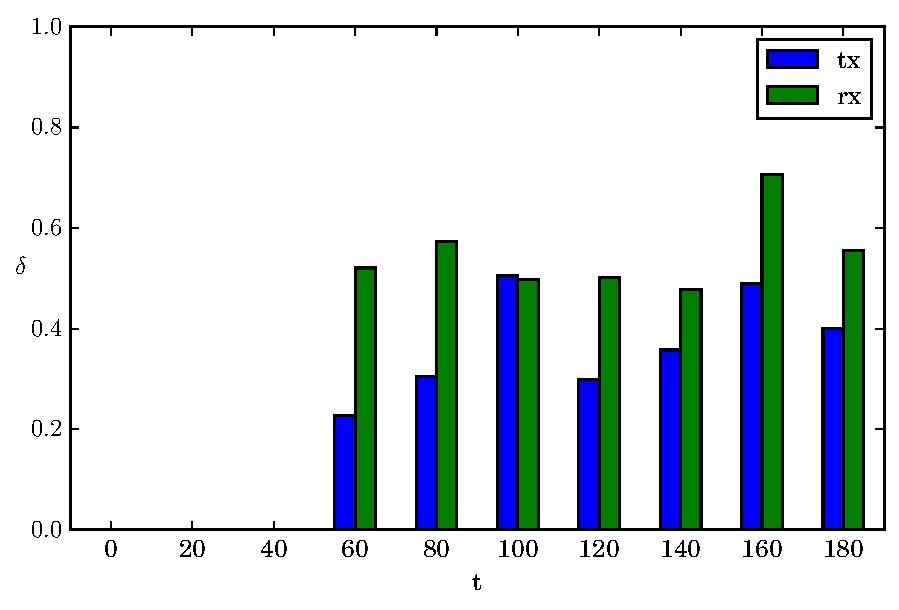
\includegraphics[width=\textwidth]{figures/evolution_route_3.pdf}
  \end{figure}
\end{frame}

\begin{frame}{$\delta(t)$ - Estimation ``maillée'' - 4}
  \begin{figure}
    \centering  
    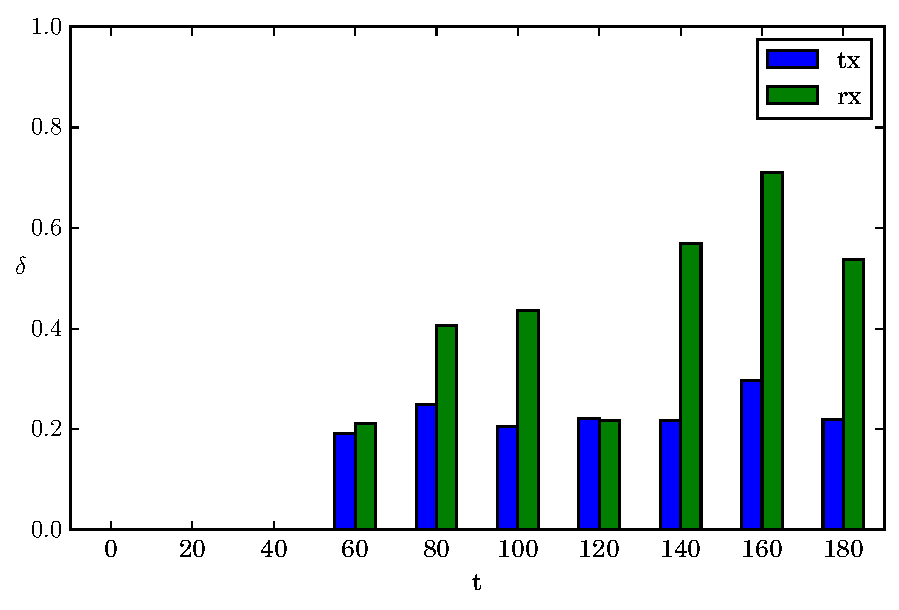
\includegraphics[width=\textwidth]{figures/evolution_route_4.pdf}
  \end{figure}
\end{frame}

\begin{frame}{$\delta(t)$ - Estimation ``maillée'' - 5}
  \begin{figure}
    \centering  
    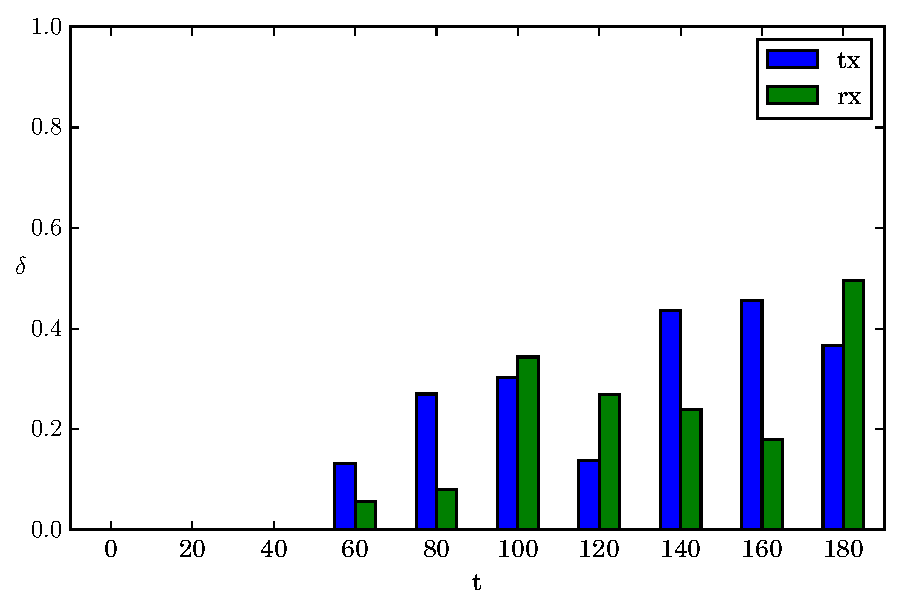
\includegraphics[width=\textwidth]{figures/evolution_route_5.pdf}
  \end{figure}
\end{frame}

\begin{frame}{$\delta(t)$ - Estimation ``maillée'' - 6}
  \begin{figure}
    \centering  
    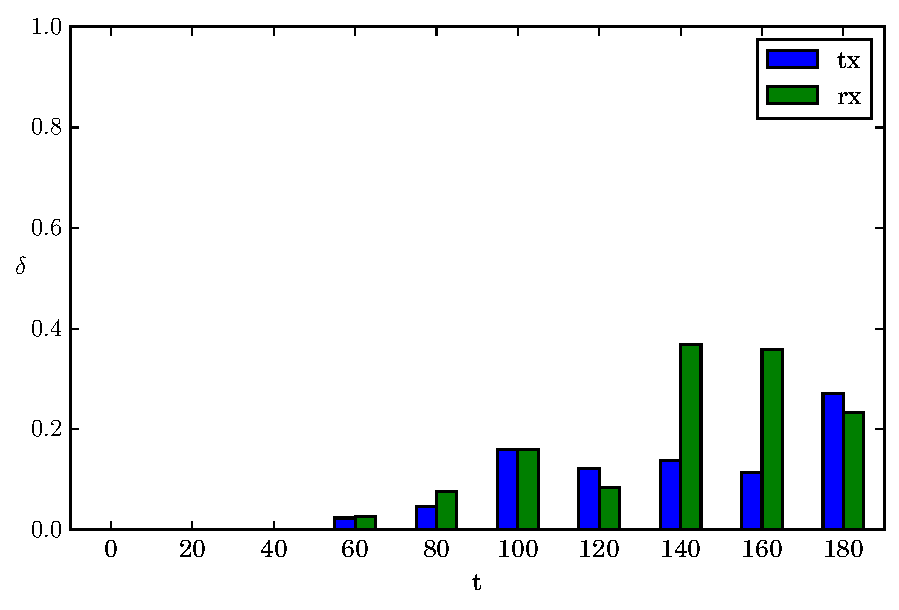
\includegraphics[width=\textwidth]{figures/evolution_route_6.pdf}
  \end{figure}
\end{frame}

\begin{frame}{Intervalle de recalibration}
  \begin{figure}[ht]
    \centering
    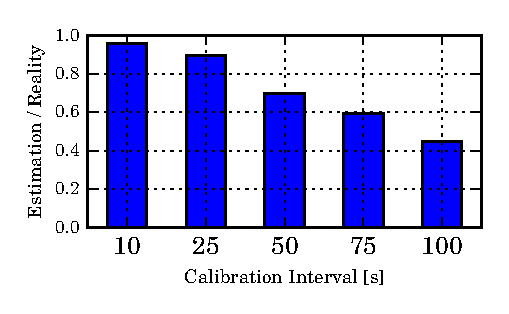
\includegraphics[width=\textwidth]{figures/ratio_recalibration.pdf}
  \end{figure}
\end{frame}

% \begin{frame}\frametitle{Estimation dans le cas multi-sauts}

%   \begin{figure}[tb]
%     \centering
%     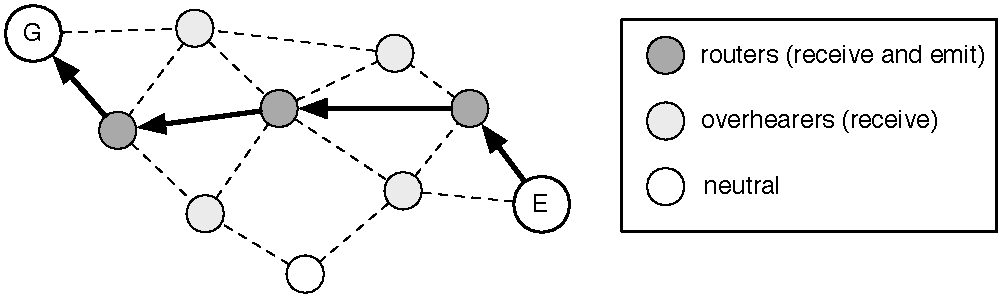
\includegraphics[scale=.6]{figures/estimators_schemaCC.pdf}
%   \end{figure}

%   \begin{block}{Estimation de la consommation énergétique}
%     % \begin{description}

%     % \item[Noinfo] $\widehat{E}_i(t) = \sum_{m \in \mathcal{D}_i(t)}{S_{\textrm{cost}}(m)} + \sum_{m \in \mathcal{A}_i(t)}{R_{\textrm{cost}}(m)}.$

%     % \item[Route]
%     $\widehat{E}_i(t) =  \sum_{m \in \mathcal{D}_i(t) \cup \mathcal{F}_i(t)}{S_{\textrm{cost}}(m)} + \sum_{m \in \mathcal{A}_i(t) \cup \mathcal{F}_i(t)}{R_{\textrm{cost}}(m)}$

%     % \end{description}
%   \end{block}

% \end{frame}
